\documentclass[11pt,a4paper]{article}

\usepackage[utf8]{inputenc}
\usepackage[T1]{fontenc}
\usepackage[frenchb]{babel}
\usepackage{amsmath,amssymb,amsfonts}
\usepackage{graphicx}
\usepackage{booktabs}
\usepackage[margin=2.4cm]{geometry}
\usepackage{caption}
\usepackage{float}
\usepackage[colorlinks=false,pdfborder={0 0 0}]{hyperref}

\graphicspath{{figures/}}

\newcommand{\R}{\mathbb{R}}
\newcommand{\E}{\mathbb{E}}
\newcommand{\pfrac}[2]{\frac{\partial #1}{\partial #2}}
\newcommand{\norm}[1]{\left\lVert #1 \right\rVert}
\newcommand{\vect}[1]{\mathbf{#1}}
\newcommand{\diag}{\operatorname{diag}}

% Renseigner ici vos informations
\newcommand{\NomEtudiant}{YAMBOGO Brice}
\newcommand{\Classe}{S7 --- Optimisation pour le Machine Learning}

\title{\textbf{MiniNet-Opt}\\[4pt]
\large Conception, entraînement, régularisation et optimisation sous contraintes d'un réseau de neurones}
\author{\NomEtudiant\\[2pt] \Classe}
\date{\today}

\begin{document}

\maketitle

\begin{abstract}
Ce rapport présente la conception complète, de bout en bout, d'un réseau de neurones multicouche de classification binaire entièrement implémenté en \textsc{NumPy} (sans autodifférence), son entraînement par trois méthodes de gradient (SGD, Momentum, Adam), le contrôle de sa généralisation par trois techniques de régularisation ($L_2$, dropout, early stopping) et sa reformulation comme problème d'optimisation sous contrainte résolu par gradient projeté. Chaque brique est validée numériquement (gradient checking, comparaison à PyTorch) et chaque choix est justifié par un protocole expérimental reproductible : graines fixées, découpage train/validation/test strict, sélection des hyperparamètres sur validation uniquement et évaluation unique finale sur test. Les résultats montrent que les trois optimiseurs atteignent des performances comparables (accuracy de test $0{,}957$--$0{,}967$), que l'early stopping et la pénalité $L_2$ réduisent efficacement l'écart train/validation, et qu'une contrainte explicite $\norm{\theta}_2 \le R$ n'affecte la solution que lorsque $R$ est inférieur à la norme naturelle des paramètres, auquel cas la pénalisation et la contrainte conduisent à des solutions distinctes, la contrainte étant plus restrictive.
\end{abstract}

\tableofcontents

\section{Introduction et problème étudié}
\label{sec:intro}

L'entraînement d'un réseau de neurones peut être vu comme un problème d'optimisation paramétrique. On note $\theta = \bigl(\vect{W}^{(1)}, \vect{b}^{(1)}, \dots, \vect{W}^{(L)}, \vect{b}^{(L)}\bigr)$ l'ensemble des paramètres du réseau et
\[
F_{\mathrm{train}}(\theta) = \frac{1}{n} \sum_{i=1}^{n} \ell\bigl(f_\theta(\vect{x}_i), y_i\bigr)
\]
la perte empirique sur l'échantillon d'entraînement $\mathcal{D}_{\mathrm{train}} = \{(\vect{x}_i, y_i)\}_{i=1}^n$. Le projet \emph{MiniNet-Opt} enrichit progressivement ce problème selon trois points de vue :

\begin{enumerate}
  \item \textbf{Optimisation} : résoudre $\min_\theta F_{\mathrm{train}}(\theta)$ par différentes méthodes de gradient et comparer leur convergence ;
  \item \textbf{Régularisation} : résoudre $\min_\theta F_{\mathrm{train}}(\theta) + \lambda \Omega(\theta)$ et contrôler la généralisation hors échantillon ;
  \item \textbf{Optimisation sous contraintes} : résoudre $\min_\theta F_{\mathrm{train}}(\theta)$ sous la contrainte $\theta \in \mathcal{C}$, ici $\mathcal{C} = \{\theta : \norm{\theta}_2 \le R\}$, par gradient projeté.
\end{enumerate}

Le fil conducteur est donc : \emph{construire un réseau} $\to$ \emph{l'optimiser} $\to$ \emph{contrôler sa généralisation} $\to$ \emph{imposer des contraintes explicites}. Le but n'est pas seulement d'obtenir une bonne précision de classification, mais de \emph{comprendre expérimentalement et mathématiquement} les mécanismes qui gouvernent l'entraînement. Conformément à l'exigence du sujet, la première version du réseau et des optimiseurs est programmée en \textsc{NumPy}, sans autograd ; PyTorch n'est utilisé qu'en fin de projet comme référence de vérification.

Le rapport suit la structure recommandée par le sujet et répond explicitement aux douze questions scientifiques de la section~\ref{sec:questions}. Les résultats intermédiaires de toutes les expériences sont enregistrés dans \texttt{results/summary.json} et les tableaux du rapport sont générés automatiquement par le code (\texttt{results/tables.tex}), ce qui garantit la cohérence entre le texte, les figures et les expériences.

\section{Données et protocole expérimental}
\label{sec:data}

\subsection{Jeu de données}

Le problème étudié est la classification binaire sur le jeu de données \texttt{make\_moons} de \texttt{scikit-learn} :
\[
X, y = \texttt{make\_moons}(\texttt{n\_samples}=1500,\ \texttt{noise}=0{,}20,\ \texttt{random\_state}=42).
\]
La matrice $X \in \R^{1500 \times 2}$ contient les coordonnées $x_1, x_2$ de chaque point ; le vecteur $y \in \{0,1\}^{1500}$ contient les étiquettes. Les deux classes sont des croissants imbriqués, ce qui rend le problème \emph{non linéairement séparable} : un réseau à couches cachées est nécessaire.

\subsection{Découpage train / validation / test}

Les données sont divisées en trois ensembles disjoints par permutation aléatoire reproductible (graine $42$) :
\begin{itemize}
  \item entraînement $\mathcal{D}_{\mathrm{train}}$ : $60\,\%$, soit $n_{\mathrm{train}} = 900$ exemples ;
  \item validation $\mathcal{D}_{\mathrm{val}}$ : $20\,\%$, soit $n_{\mathrm{val}} = 300$ exemples ;
  \item test $\mathcal{D}_{\mathrm{test}}$ : $20\,\%$, soit $n_{\mathrm{test}} = 300$ exemples.
\end{itemize}
Le jeu de validation sert exclusivement à la sélection des hyperparamètres (taux d'apprentissage, $\lambda$, taux de dropout, nombre d'époques) ; le jeu de test n'est évalué qu'une seule fois, en fin de protocole, sur les modèles déjà sélectionnés.

\subsection{Standardisation}

Les entrées sont standardisées avec les statistiques du jeu d'entraînement \emph{uniquement}, afin de ne pas faire fuiter d'information des jeux de validation et de test :
\[
x \mapsto \frac{x - \mu_{\mathrm{train}}}{\sigma_{\mathrm{train}}},
\qquad \mu_{\mathrm{train}} = \frac{1}{n_{\mathrm{train}}} \sum_{i} x_i,\qquad
\sigma^2_{\mathrm{train}} = \frac{1}{n_{\mathrm{train}}} \sum_{i} (x_i - \mu_{\mathrm{train}})^2.
\]
Cette standardisation centrée-réduite facilite l'optimisation (gradients mieux conditionnés, taux d'apprentissage homogènes selon les axes).

\subsection{Reproductibilité}

Toutes les sources d'aléa sont contrôlées par des graines fixées : génération des données (graine $42$), découpage (graine $42$), initialisation des poids (graines $42$, $7$ et $123$ selon l'expérience) et tirage des mini-batchs (graine $42$). La figure~\ref{fig:data} visualise les trois découpages ; la balance des classes dans le jeu d'entraînement est de $52{,}2\,\%$ (classes quasi équilibrées).

\begin{figure}[H]
\centering
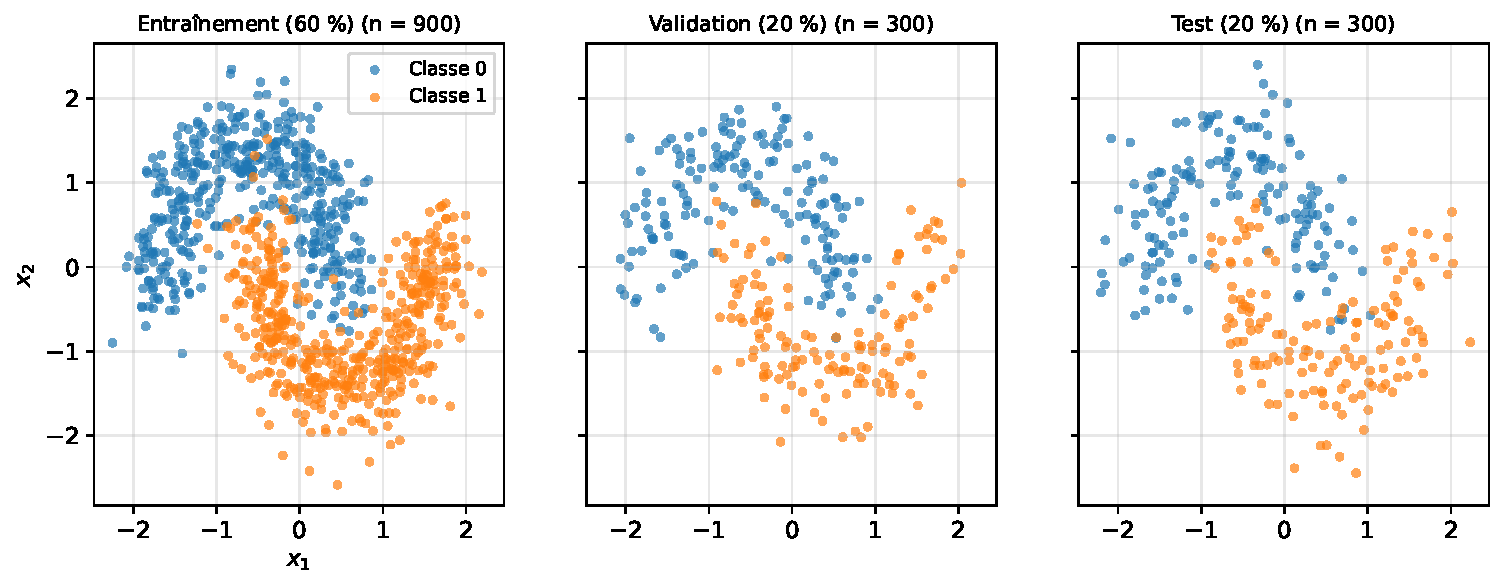
\includegraphics[width=\textwidth]{a1_data.pdf}
\caption{Données \texttt{make\_moons} ($n=1500$, bruit $0{,}20$) et découpage train/validation/test après standardisation.}
\label{fig:data}
\end{figure}

\section{Architecture du réseau}
\label{sec:archi}

On considère le réseau multicouche de classification binaire imposé par le sujet :
\[
d \;\longrightarrow\; n_1 \;\longrightarrow\; n_2 \;\longrightarrow\; 1,
\qquad
2 \to 16 \to 8 \to 1 .
\]
Les couches cachées utilisent l'activation ReLU, $\mathrm{ReLU}(z) = \max(0, z)$, et la sortie utilise la sigmoïde $\sigma(z) = \frac{1}{1+e^{-z}}$, ce qui donne $\hat y = \sigma(z^{(3)}) \in (0,1)$ interprété comme la probabilité $P(Y=1 \mid x)$. Le réseau comporte donc trois couches affines : $\vect{W}^{(1)} \in \R^{16 \times 2}$, $\vect{b}^{(1)} \in \R^{16}$ ; $\vect{W}^{(2)} \in \R^{8 \times 16}$, $\vect{b}^{(2)} \in \R^{8}$ ; $\vect{W}^{(3)} \in \R^{1 \times 8}$, $\vect{b}^{(3)} \in \R$, soit $193$ paramètres au total ($32 + 16 + 128 + 8 + 8 + 1$).

\subsection{Propagation avant}

Pour une observation $\vect{x} \in \R^d$, la propagation avant s'écrit
\begin{align}
\vect{z}^{(1)} &= \vect{W}^{(1)} \vect{x} + \vect{b}^{(1)}, &
\vect{a}^{(1)} &= \mathrm{ReLU}(\vect{z}^{(1)}), \label{eq:fwd1}\\
\vect{z}^{(2)} &= \vect{W}^{(2)} \vect{a}^{(1)} + \vect{b}^{(2)}, &
\vect{a}^{(2)} &= \mathrm{ReLU}(\vect{z}^{(2)}), \label{eq:fwd2}\\
z^{(3)} &= \vect{W}^{(3)} \vect{a}^{(2)} + b^{(3)}, &
\hat y &= \sigma(z^{(3)}). \label{eq:fwd3}
\end{align}
Les couches ReLU et sigmoïde s'appliquent composante par composante.

\subsection{Fonction de perte}

La perte utilisée est la \emph{binary cross-entropy} :
\[
\ell(\hat y, y) = -y \ln \hat y - (1-y) \ln (1-\hat y),
\]
et la perte empirique sur un mini-batch $\mathcal{B}$ est
\[
F_{\mathcal{B}}(\theta) = \frac{1}{|\mathcal{B}|} \sum_{i \in \mathcal{B}} \ell(\hat y_i, y_i).
\]

\subsection{Initialisation des poids}

Les poids sont initialisés selon l'initialisation de He \cite{he2015}, adaptée aux activations ReLU :
\[
W^{(l)}_{ij} \sim \mathcal{N}\Bigl(0, \tfrac{2}{n_{l-1}}\Bigr),
\qquad b^{(l)} = 0,
\]
où $n_{l-1}$ est le nombre de neurones de la couche précédente. Cette initialisation conserve la variance des activations à travers les couches et évite l'explosion ou la disparition des gradients en début d'entraînement.

\subsection{Implémentation}

Le dépôt suit l'architecture logicielle recommandée par le sujet :
\texttt{data.py} (génération, découpage, standardisation), \texttt{layers.py} (\texttt{Linear}, \texttt{ReLU}, \texttt{Sigmoid}, \texttt{Dropout}), \texttt{model.py} (assemblage du réseau), \texttt{losses.py} (BCE et son gradient), \texttt{optimizers.py} (SGD, Momentum, Adam), \texttt{regularization.py} ($L_2$, early stopping), \texttt{constraints.py} (norme, projection, gradient projeté), \texttt{train.py} (boucle d'entraînement), \texttt{experiments.py} (protocoles), \texttt{plots.py} (visualisations), \texttt{torch\_verify.py} (vérification PyTorch) et \texttt{main.py} (point d'entrée). Chaque couche mémorise les quantités intermédiaires du forward nécessaires au backward, conformément à l'exigence du sujet.

\section{Rétropropagation et vérification des gradients}
\label{sec:backprop}

\subsection{Dérivées des activations}

Les activations sont dérivables presque partout :
\[
\mathrm{ReLU}'(z) = \mathbf{1}_{\{z > 0\}},
\qquad
\sigma'(z) = \sigma(z)\bigl(1 - \sigma(z)\bigr).
\]

\subsection{Gradient de la perte par rapport à la sortie}

Pour un couple $(\hat y, y)$, en utilisant $\hat y = \sigma(z^{(3)})$ :
\[
\frac{\partial \ell}{\partial \hat y} = \frac{\hat y - y}{\hat y (1-\hat y)},
\qquad
\frac{\partial \ell}{\partial z^{(3)}} = \frac{\partial \ell}{\partial \hat y} \cdot \sigma'(z^{(3)}) = \hat y - y .
\]
Pour un mini-batch $\mathcal{B}$ de taille $m$, on pose, par composante de sortie :
\[
\vect{\delta}^{(3)} = \pfrac{F_{\mathcal{B}}}{z^{(3)}} = \frac{1}{m} \bigl( \hat{\vect y} - \vect{y} \bigr).
\]

\subsection{Relations récursives de la rétropropagation}

En notant $\vect{\delta}^{(l)} = \pfrac{F_{\mathcal{B}}}{\vect{z}^{(l)}}$, la règle de chaîne donne les relations récursives (propagées de la couche de sortie vers l'entrée) :
\begin{align}
\vect{\delta}^{(2)} &= \bigl(\vect{W}^{(3)}\bigr)^\top \vect{\delta}^{(3)} \;\odot\; \mathrm{ReLU}'\bigl(\vect{z}^{(2)}\bigr), \label{eq:rec2}\\
\vect{\delta}^{(1)} &= \bigl(\vect{W}^{(2)}\bigr)^\top \vect{\delta}^{(2)} \;\odot\; \mathrm{ReLU}'\bigl(\vect{z}^{(1)}\bigr), \label{eq:rec1}
\end{align}
où $\odot$ désigne le produit composante par composante (Hadamard) et où les masques $\mathrm{ReLU}'(\vect{z}^{(l)})$ sont directement les masques binaires $\mathbf{1}_{\{\vect{z}^{(l)} > 0\}}$ stockés lors du forward.

\subsection{Gradients des poids et des biais}

La couche affine $\vect{z}^{(l)} = \vect{W}^{(l)} \vect{a}^{(l-1)} + \vect{b}^{(l)}$ (avec la convention $\vect{a}^{(0)} = \vect{x}$) a pour gradients :
\begin{align}
\pfrac{F_{\mathcal{B}}}{\vect{W}^{(l)}} &= \frac{1}{m} \sum_{i \in \mathcal{B}} \vect{\delta}_i^{(l)} \, \bigl(\vect{a}_i^{(l-1)}\bigr)^\top, \label{eq:gradW}\\
\pfrac{F_{\mathcal{B}}}{\vect{b}^{(l)}} &= \frac{1}{m} \sum_{i \in \mathcal{B}} \vect{\delta}_i^{(l)} . \label{eq:gradb}
\end{align}
En écriture matricielle, avec les notations du code : $\pfrac{F_{\mathcal{B}}}{\vect{W}^{(l)}} = \bigl(\Delta^{(l)}\bigr)^\top A^{(l-1)} / m$, et $\pfrac{F_{\mathcal{B}}}{\vect{b}^{(l)}}$ est la moyenne de $\Delta^{(l)}$ sur les lignes.

\subsection{Gradient de la pénalité $L_2$}

Pour la version régularisée $F_\lambda(\theta) = F_{\mathrm{train}}(\theta) + \frac{\lambda}{2} \sum_{l} \norm{\vect{W}^{(l)}}_F^2$ (les biais n'étant pas pénalisés), le gradient s'obtient par linéarité :
\[
\pfrac{}{\vect{W}^{(l)}} \Bigl( \tfrac{\lambda}{2} \norm{\vect{W}^{(l)}}_F^2 \Bigr) = \lambda \vect{W}^{(l)}.
\]

\subsection{Gradient du dropout}

Le dropout inversé remplace pendant l'entraînement l'activation $\vect{h}$ par $\tilde{\vect{h}} = \frac{\vect{M}}{p} \odot \vect{h}$ où $M_j \sim \mathrm{Bernoulli}(p)$ (conservation avec probabilité $p$). La multiplication par $\frac{1}{p}$ garantit $\E[\tilde{\vect{h}}] = \vect{h}$, de sorte qu'en validation et en test (dropout désactivé), l'échelle des activations est inchangée. En rétropropagation, le gradient est multiplié par le même masque : $\frac{\partial \tilde h_j}{\partial h_j} = \frac{M_j}{p}$.

\subsection{Vérification numérique par différences finies}

Avant tout entraînement, le backward est validé par différences finies centrées. Pour chaque composante $\theta_j$ :
\[
\pfrac{F}{\theta_j} \approx \frac{F(\theta + \varepsilon \vect{e}_j) - F(\theta - \varepsilon \vect{e}_j)}{2\varepsilon},
\qquad \varepsilon = 10^{-5},
\]
et l'erreur relative est mesurée par
\[
\mathrm{err} = \frac{\norm{\vect{g}_{\text{analytique}} - \vect{g}_{\text{numérique}}}}{\norm{\vect{g}_{\text{analytique}}} + \norm{\vect{g}_{\text{numérique}}} + \varepsilon}.
\]
Le tableau~\ref{tab:gradcheck} (inclus depuis \texttt{results/tables.tex}, généré par le code) montre des erreurs relatives de l'ordre de $10^{-11}$, très inférieures au seuil usuel de $10^{-6}$ : la rétropropagation est exacte, aux erreurs d'arrondi près.

% Tableaux générés automatiquement par experiments.py
% Ne pas éditer à la main.

\begin{table}[htbp]
\centering
\caption{Erreurs relatives du gradient checking (différences finies centrées, $\varepsilon = 10^{-5}$).}
\label{tab:gradcheck}
\resizebox{\textwidth}{!}{\begin{tabular}{lccccccc}
\toprule
 & $W^{(1)}$ & $b^{(1)}$ & $W^{(2)}$ & $b^{(2)}$ & $W^{(3)}$ & $b^{(3)}$ & Maximum \\
\midrule
Erreur relative & $4.4\times 10^{-11}$ & $2.7\times 10^{-11}$ & $1.9\times 10^{-11}$ & $4.9\times 10^{-11}$ & $2.8\times 10^{-11}$ & $1.8\times 10^{-12}$ & $4.9\times 10^{-11}$ \\
\bottomrule
\end{tabular}}
\end{table}


\begin{table}[htbp]
\centering
\caption{Comparaison SGD / Momentum / Adam (moyenne $\pm$ écart-type sur 3 graines, 300 époques, batch 32).}
\label{tab:c}
\resizebox{\textwidth}{!}{\begin{tabular}{llccccc}
\toprule
Optimiseur & Hyperparamètres & \multicolumn{1}{c}{Loss train} & \multicolumn{1}{c}{Loss val.} & \multicolumn{1}{c}{Acc. val.} & \multicolumn{1}{c}{1\textsuperscript{re} époque acc $\ge 0{,}95$} & \multicolumn{1}{c}{Temps (s)} \\
\midrule
SGD & $\alpha = 0{,}1$ & 0.0667 $\pm$ 0.0008 & 0.0847 $\pm$ 0.0037 & 0.974 $\pm$ 0.002 & 18.7 $\pm$ 5.2 & 2.13 $\pm$ 0.78 \\
Momentum & $\alpha = 0{,}1$, $\beta = 0{,}9$ & 0.0676 $\pm$ 0.0013 & 0.0898 $\pm$ 0.0083 & 0.974 $\pm$ 0.002 & 17.7 $\pm$ 3.3 & 3.26 $\pm$ 0.10 \\
Adam & $\alpha = 10^{-3}$ & 0.0686 $\pm$ 0.0006 & 0.0821 $\pm$ 0.0020 & 0.977 $\pm$ 0.000 & 47.3 $\pm$ 11.9 & 4.36 $\pm$ 0.23 \\
\bottomrule
\end{tabular}}
\end{table}


\begin{table}[htbp]
\centering
\caption{Sensibilité au pas d'apprentissage $\alpha$ et au paramètre $\beta$ du momentum (300 époques, batch 32).}
\label{tab:c_lr}
\resizebox{\textwidth}{!}{\begin{tabular}{lcccc}
\toprule
Configuration & Loss train & Loss val. & Acc. val. & $\|\theta^\star\|_2$ \\
\midrule
SGD ($\alpha = 0.001$) & 0.2573 & 0.2995 & 0.877 & 6.375 \\
SGD ($\alpha = 0.01$) & 0.1070 & 0.1075 & 0.963 & 7.588 \\
SGD ($\alpha = 0.1$) & 0.0665 & 0.0805 & 0.973 & 9.425 \\
SGD ($\alpha = 1$) & 0.0601 & 0.1411 & 0.977 & 16.922 \\
Adam ($\alpha = 0.0001$) & 0.2061 & 0.2326 & 0.900 & 6.811 \\
Adam ($\alpha = 0.001$) & 0.0687 & 0.0842 & 0.977 & 9.572 \\
Adam ($\alpha = 0.01$) & 0.0547 & 0.1311 & 0.977 & 17.394 \\
Adam ($\alpha = 0.1$) & 0.0784 & 0.1900 & 0.967 & 43.694 \\
Momentum ($\beta = 0.5$) & 0.0662 & 0.0804 & 0.977 & 9.454 \\
Momentum ($\beta = 0.9$) & 0.0657 & 0.0814 & 0.977 & 9.355 \\
Momentum ($\beta = 0.99$) & 0.0694 & 0.0798 & 0.977 & 8.898 \\
\bottomrule
\end{tabular}}
\end{table}


\begin{table}[htbp]
\centering
\caption{Effet de la pénalité $L_2$ (Adam, 300 époques) : les biais ne sont pas pénalisés.}
\label{tab:d_l2}
\resizebox{\textwidth}{!}{\begin{tabular}{lccccc}
\toprule
Pénalité & Loss train & Loss val. & Acc. val. & $\|\theta^\star\|_2$ & Écart val. $-$ train \\
\midrule
$\lambda = 0$ & 0.0687 & 0.0842 & 0.977 & 9.572 & 0.016 \\
$\lambda = 0.00001$ & 0.0679 & 0.0883 & 0.977 & 9.592 & 0.020 \\
$\lambda = 0.0001$ & 0.0689 & 0.0868 & 0.977 & 9.009 & 0.018 \\
$\lambda = 0.001$ & 0.0740 & 0.0786 & 0.977 & 7.232 & 0.005 \\
$\lambda = 0.01$ & 0.1161 & 0.1233 & 0.963 & 4.805 & 0.007 \\
$\lambda = 0.1$ & 0.3104 & 0.3459 & 0.857 & 2.020 & 0.036 \\
\bottomrule
\end{tabular}}
\end{table}


\begin{table}[htbp]
\centering
\caption{Effet du dropout (taux $\delta = 1-p$), Adam, 300 époques. Le dropout est désactivé en validation.}
\label{tab:d_dropout}
\resizebox{\textwidth}{!}{\begin{tabular}{lcccc}
\toprule
Conservation $p$ & Loss train & Loss val. & Acc. val. & Écart val. $-$ train \\
\midrule
$p = 0.9$ & 0.0724 & 0.0929 & 0.977 & 0.021 \\
$p = 0.8$ & 0.0818 & 0.1035 & 0.970 & 0.022 \\
$p = 0.7$ & 0.1011 & 0.1306 & 0.963 & 0.029 \\
$p = 0.5$ & 0.1770 & 0.2022 & 0.913 & 0.025 \\
\bottomrule
\end{tabular}}
\end{table}


\begin{table}[htbp]
\centering
\caption{Évaluation finale unique sur le jeu de test des modèles sélectionnés par validation.}
\label{tab:d_test}
\resizebox{\textwidth}{!}{\begin{tabular}{lccccc}
\toprule
Modèle sélectionné & Hyperparamètre & Loss train & Loss val. & Loss test & Acc. test \\
\midrule
Sans régularisation & -- & 0.0687 & 0.0842 & 0.0960 & 0.957 \\
Pénalité $L_2$ & $\lambda = 0.001$ & 0.0740 & 0.0786 & 0.0919 & 0.957 \\
Dropout & $p = 0.9$ & 0.0724 & 0.0929 & 0.1030 & 0.963 \\
Early stopping & patience $= 20$ & 0.0784 & 0.0762 & 0.0939 & 0.957 \\
\bottomrule
\end{tabular}}
\end{table}


\begin{table}[htbp]
\centering
\caption{Gradient projeté (Adam projeté sur la boule $\|\theta\|_2 \le R$). $R_0$ est la norme de la solution non contrainte de référence. $r_{\mathrm{feas}}$ est le maximum par époque de la violation avant projection.}
\label{tab:e}
\resizebox{\textwidth}{!}{\begin{tabular}{lccccccl}
\toprule
Contrainte & Loss train & Loss val. & Acc. val. & $\|\theta^\star\|_2$ & $r_{\mathrm{feas}}$ & Contrainte \\
\midrule
$R = 0.5R_0$ (4.786) & 0.1941 & 0.2138 & 0.913 & 4.786 & 1.2715 & oui \\
$R = 0.75R_0$ (7.179) & 0.0784 & 0.0855 & 0.977 & 7.179 & 0.0040 & oui \\
$R = 1R_0$ (9.572) & 0.0687 & 0.0842 & 0.977 & 9.571 & 0.0002 & oui \\
$R = 1.5R_0$ (14.358) & 0.0687 & 0.0842 & 0.977 & 9.572 & 0.0000 & non \\
$R = 2R_0$ (19.144) & 0.0687 & 0.0842 & 0.977 & 9.572 & 0.0000 & non \\
\bottomrule
\end{tabular}}
\end{table}


\begin{table}[htbp]
\centering
\caption{Comparaison pénalisation $L_2$ contre contrainte explicite $\|\theta\|_2 \le R$ à normes finales comparables (moyenne $\pm$ écart-type sur 3 graines).}
\label{tab:f}
\resizebox{\textwidth}{!}{\begin{tabular}{lccccccc}
\toprule
Pénalité & Rayon $R$ & \multicolumn{1}{c}{Loss val. (pén.)} & \multicolumn{1}{c}{Loss val. (cont.)} & \multicolumn{1}{c}{Acc. test (pén.)} & \multicolumn{1}{c}{Acc. test (cont.)} & \multicolumn{1}{c}{$\|\theta^\star\|$ (pén.)} & \multicolumn{1}{c}{$\|\theta^\star\|$ (cont.)} \\
\midrule
$\lambda = 0.0001$ & $R = 9.009$ & 0.0828 $\pm$ 0.0029 & 0.0806 $\pm$ 0.0014 & 0.960 $\pm$ 0.000 & 0.960 $\pm$ 0.003 & 9.192 & 9.009 \\
$\lambda = 0.001$ & $R = 7.232$ & 0.0794 $\pm$ 0.0008 & 0.0870 $\pm$ 0.0015 & 0.959 $\pm$ 0.002 & 0.961 $\pm$ 0.006 & 7.295 & 7.232 \\
$\lambda = 0.01$ & $R = 4.805$ & 0.1233 $\pm$ 0.0009 & 0.2232 $\pm$ 0.0087 & 0.950 $\pm$ 0.000 & 0.910 $\pm$ 0.005 & 4.837 & 4.805 \\
\bottomrule
\end{tabular}}
\end{table}


\begin{table}[htbp]
\centering
\caption{Vérification PyTorch : mêmes initialisations, mêmes lots, mêmes hyperparamètres (float64).}
\label{tab:g}
\resizebox{\textwidth}{!}{\begin{tabular}{lcccccc}
\toprule
Optimiseur & Cadre & Loss train & Loss val. & Acc. val. & Acc. test & Max $|\Delta$loss$|$ \\
\midrule
SGD & NumPy & 0.0665 & 0.0805 & 0.973 & 0.967 & -- \\
SGD & PyTorch & 0.0665 & 0.0805 & 0.973 & 0.967 & $5.7\times 10^{-11}$ \\

Adam & NumPy & 0.0687 & 0.0842 & 0.977 & 0.957 & -- \\
Adam & PyTorch & 0.0687 & 0.0842 & 0.977 & 0.957 & $1.1\times 10^{-12}$ \\
\bottomrule
\end{tabular}}
\end{table}



Enfin, la condition de validité du jalon J1 est vérifiée : sur un très petit jeu de données ($8$ exemples, SGD avec $\alpha = 0{,}5$ en batch complet), la loss décroît de $\approx 0{,}69$ vers $0{,}0029$ en $300$ époques et l'accuracy atteint $1{,}0$ (figure~\ref{fig:j1}), ce qui confirme que le réseau est capable d'apprendre.

\begin{figure}[H]
\centering
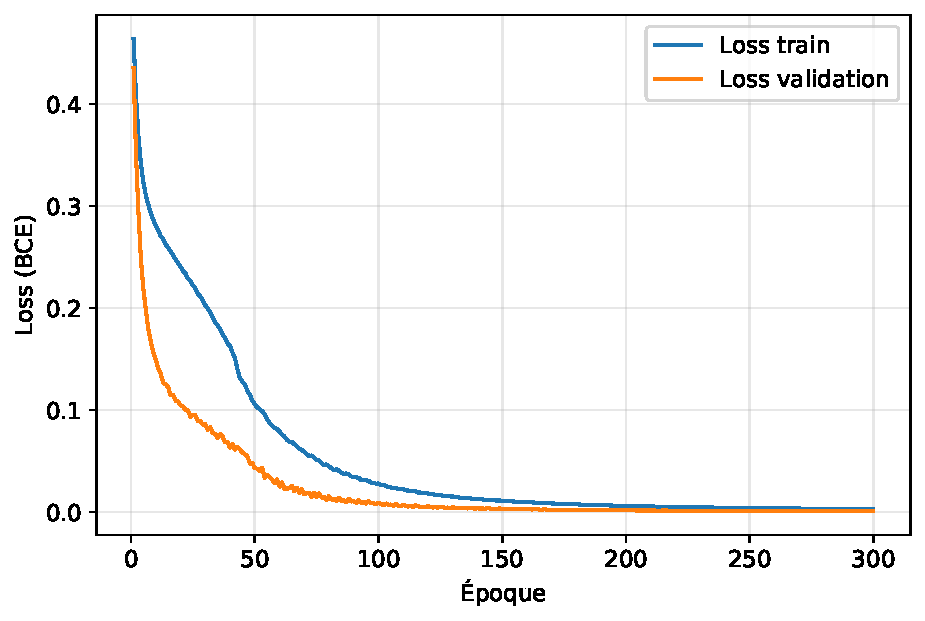
\includegraphics[width=0.62\textwidth]{j1_small_fit.pdf}
\caption{Validation J1 : la loss décroît régulièrement sur un très petit jeu de données (8 exemples).}
\label{fig:j1}
\end{figure}

\section{Méthodes d'optimisation}
\label{sec:optim}

\subsection{Algorithmes implémentés}

Les trois optimiseurs demandés sont implémentés composante par composante, sans autograd :

\textbf{SGD.} À chaque itération $k$, pour un mini-batch $\mathcal{B}_k$ :
\[
\vect{g}_k = \nabla F_{\mathcal{B}_k}(\theta_k),
\qquad
\theta_{k+1} = \theta_k - \alpha \vect{g}_k .
\]

\textbf{Momentum.} Le momentum accumule une moyenne mobile des gradients passés :
\[
\vect{v}_{k+1} = \beta \vect{v}_k + (1-\beta) \vect{g}_k,
\qquad
\theta_{k+1} = \theta_k - \alpha \vect{v}_{k+1}.
\]

\textbf{Adam.} Adam combine deux moyennes mobiles (premier et second moments) avec correction de biais :
\[
\vect{m}_k = \beta_1 \vect{m}_{k-1} + (1-\beta_1) \vect{g}_k,
\qquad
\vect{v}_k = \beta_2 \vect{v}_{k-1} + (1-\beta_2) \vect{g}_k^2,
\]
\[
\hat{\vect{m}}_k = \frac{\vect{m}_k}{1-\beta_1^k},
\qquad
\hat{\vect{v}}_k = \frac{\vect{v}_k}{1-\beta_2^k},
\qquad
\theta_{k+1} = \theta_k - \alpha \frac{\hat{\vect{m}}_k}{\sqrt{\hat{\vect{v}}_k} + \varepsilon},
\]
où $\vect{g}_k^2$, $\sqrt{\vect{v}_k}$ et la division s'effectuent composante par composante. Les hyperparamètres par défaut sont $\alpha = 10^{-3}$, $\beta_1 = 0{,}9$, $\beta_2 = 0{,}999$, $\varepsilon = 10^{-8}$.

\subsection{Protocole de comparaison}

Pour que la comparaison soit valide, tous les optimiseurs utilisent \emph{exactement} la même architecture ($2 \to 16 \to 8 \to 1$), la même initialisation des poids, le même découpage des données, les mêmes mini-batchs (même graine de tirage) et le même budget d'entraînement : $300$ époques, mini-batchs de taille $32$. Chaque expérience est répétée sur $3$ graines d'initialisation ($42$, $7$, $123$) pour estimer la variabilité. Après chaque époque sont enregistrés $F_{\mathrm{train}}(\theta_k)$, $F_{\mathrm{val}}(\theta_k)$, $\norm{\nabla F(\theta_k)}$, l'accuracy train/validation et $\norm{\theta_k}_2$.

\subsection{Résultats}

Le tableau~\ref{tab:c} et les figures~\ref{fig:c_loss}, \ref{fig:c_acc} et \ref{fig:c_grad} résument la comparaison.

\begin{figure}[H]
\centering
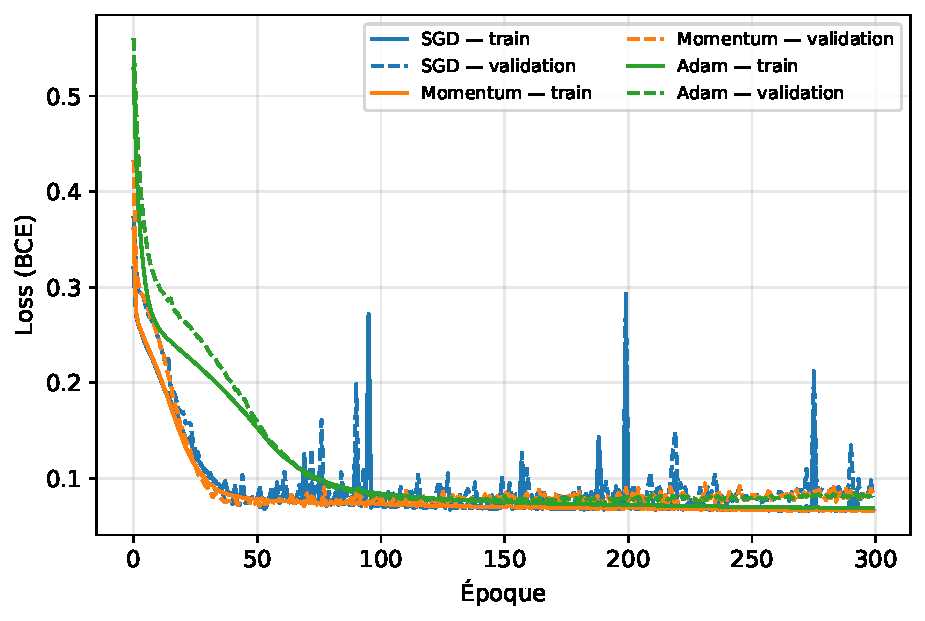
\includegraphics[width=0.72\textwidth]{c_loss.pdf}
\caption{Comparaison SGD / Momentum / Adam : loss train (trait plein) et validation (pointillés) en fonction des époques (graine 42).}
\label{fig:c_loss}
\end{figure}

\begin{figure}[H]
\centering
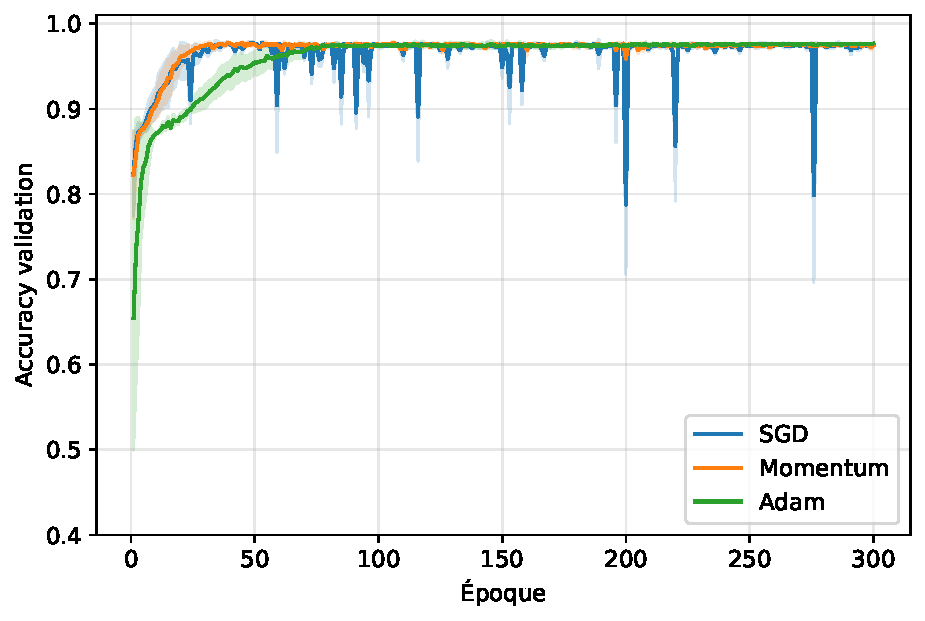
\includegraphics[width=0.62\textwidth]{c_acc.pdf}
\caption{Accuracy de validation, moyenne et écart-type sur 3 graines d'initialisation.}
\label{fig:c_acc}
\end{figure}

\begin{figure}[H]
\centering
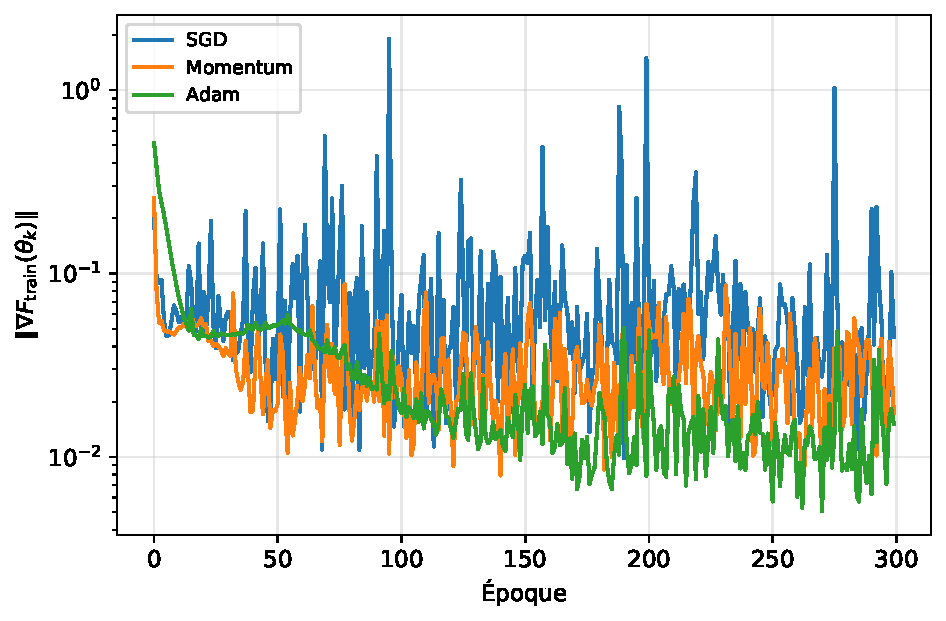
\includegraphics[width=0.72\textwidth]{c_grad.pdf}
\caption{Norme du gradient $\norm{\nabla F_{\mathrm{train}}(\theta_k)}$ (échelle logarithmique) en fonction des époques.}
\label{fig:c_grad}
\end{figure}

\textbf{Vitesse initiale.} À la première époque, la loss train vaut $0{,}336$ pour SGD, $0{,}374$ pour Momentum et $0{,}615$ pour Adam ; à la cinquième époque, $0{,}231$, $0{,}237$ et $0{,}352$ respectivement. SGD et Momentum réduisent donc la loss nettement plus vite au départ : SGD atteint une accuracy de validation $\ge 0{,}95$ en $18{,}7 \pm 5{,}2$ époques, Momentum en $17{,}7 \pm 3{,}3$, tandis qu'Adam (avec $\alpha = 10^{-3}$) met $47{,}3 \pm 11{,}9$ époques. Ce décalage est attendu : avec $\alpha = 10^{-3}$ et les corrections de biais, les premiers pas d'Adam sont petits, alors que le pas $\alpha = 0{,}1$ du SGD est bien adapté à ce problème standardisé.

\textbf{Stabilité.} Les trois courbes sont stables ; aucun optimiseur ne diverge sur cette plage d'hyperparamètres. La norme du gradient (figure~\ref{fig:c_grad}) décroît de $\sim 10^{0}$ vers $10^{-3}$--$10^{-2}$ : les trois méthodes atteignent un voisinage d'un point stationnaire, sans pathologie de gradient explosif.

\textbf{Valeur finale.} Les pertes finales sont très proches : loss train $0{,}0667$ (SGD), $0{,}0676$ (Momentum), $0{,}0686$ (Adam). Sur la validation, Adam obtient la meilleure loss ($0{,}0821$) et la meilleure accuracy ($0{,}977$), suivi de SGD ($0{,}0847$ ; $0{,}974$). L'écart-type sur 3 graines est faible ($\le 0{,}008$ en loss, $\le 0{,}002$ en accuracy) : les conclusions sont robustes au tirage des poids initiaux.

\textbf{Sensibilité au learning rate.} Le tableau~\ref{tab:c_lr} et la figure~\ref{fig:c_lr} montrent le comportement classique : un $\alpha$ trop petit ralentit l'entraînement (SGD avec $\alpha = 10^{-3}$ : accuracy $0{,}877$ ; Adam avec $\alpha = 10^{-4}$ : $0{,}900$), tandis qu'un $\alpha$ trop grand provoque du sur-apprentissage : SGD avec $\alpha = 1$ atteint une loss train de $0{,}0601$ mais une loss validation de $0{,}1411$ (norme des poids $16{,}9$), et Adam avec $\alpha = 10^{-2}$ une loss train de $0{,}0547$ pour $0{,}1311$ en validation (norme $17{,}4$). Adam se révèle plus sensible : son adaptation par composante permet de pousser la loss train plus bas, au prix d'un écart train/validation plus grand. Le paramètre $\beta$ du momentum a en revanche peu d'influence ($0{,}5$, $0{,}9$, $0{,}99$ donnent tous une accuracy de validation de $0{,}977$).

\begin{figure}[H]
\centering
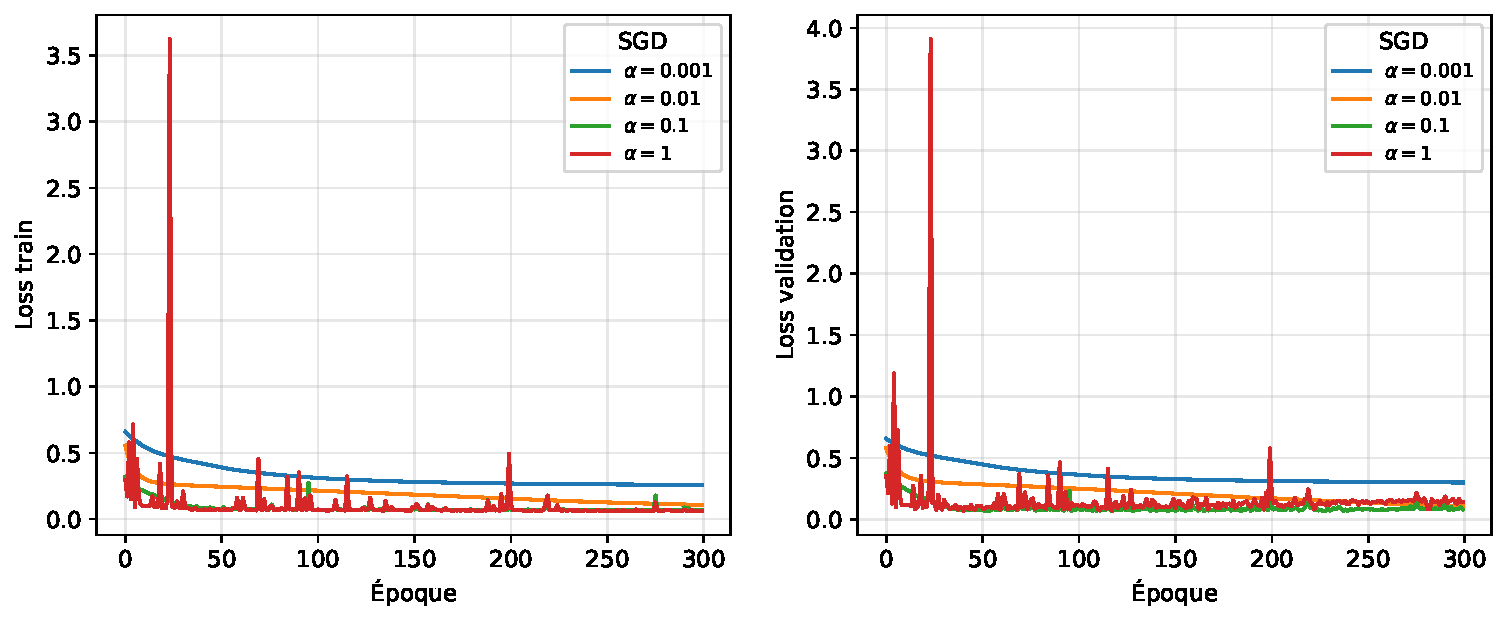
\includegraphics[width=\textwidth]{c_lr_sgd.pdf}\\[4pt]
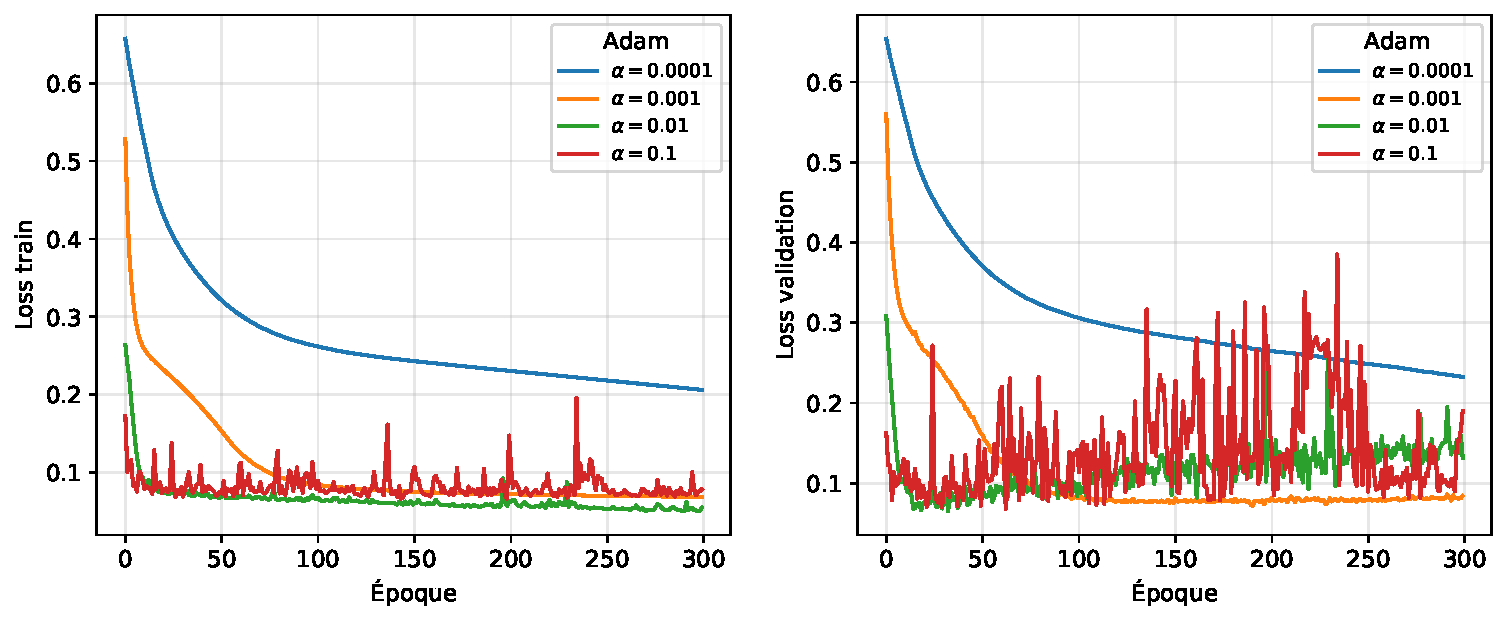
\includegraphics[width=\textwidth]{c_lr_adam.pdf}
\caption{Sensibilité au taux d'apprentissage $\alpha$ pour SGD (haut) et Adam (bas) : loss train (gauche) et validation (droite).}
\label{fig:c_lr}
\end{figure}

\textbf{Réponse à la question du sujet :} \emph{l'optimiseur qui minimise le plus vite la loss train généralise-t-il le mieux ?} Sur ce problème, non : SGD est le plus rapide à réduire la loss train, mais c'est Adam qui obtient la meilleure performance de validation finale (loss $0{,}0821$ contre $0{,}0847$). La vitesse de convergence et la qualité de la généralisation ne coïncident donc pas nécessairement ; les différences restent toutefois modestes sur ce jeu de données simple.

\section{Régularisation et généralisation}
\label{sec:reg}

\subsection{Risque empirique et performance hors échantillon}

L'entraînement minimise $F_{\mathrm{train}}(\theta)$ ; la performance de validation estime le comportement hors échantillon pendant la sélection de modèle. Le jeu de test n'est jamais consulté pour choisir l'architecture, le learning rate, le nombre d'époques, $\lambda$ ou l'optimiseur : il n'intervient qu'une seule fois, à la fin (tableau~\ref{tab:d_test}).

\subsection{Détection du sur-apprentissage}

Pour dater l'apparition du sur-apprentissage, le réseau non régularisé est entraîné $2000$ époques (figure~\ref{fig:overfit}). La loss de validation atteint son minimum à l'époque $191$ ($0{,}0714$) puis \emph{remonte} jusqu'à $0{,}2413$ en fin d'entraînement, tandis que la loss train continue de décroître jusqu'à $0{,}0489$. Le sur-apprentissage apparaît donc vers l'époque $\approx 190$ : au-delà, le réseau mémorise des particularités des $900$ exemples d'entraînement au détriment de la généralisation. Sur le budget standard de $300$ époques, l'écart train/validation reste modéré ($0{,}0155$) mais déjà visible.

\begin{figure}[H]
\centering
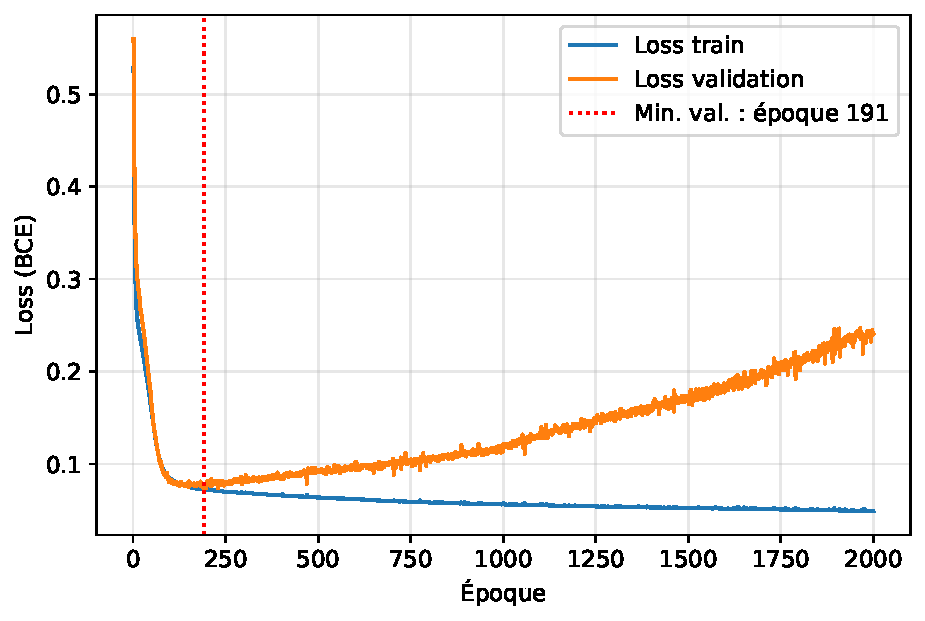
\includegraphics[width=0.72\textwidth]{d_overfit.pdf}
\caption{Sur-apprentissage : loss train et validation sur 2000 époques sans régularisation. La loss de validation se dégrade après l'époque 191.}
\label{fig:overfit}
\end{figure}

\subsection{Pénalité $L_2$}

On minimise
\[
F_\lambda(\theta) = F_{\mathrm{train}}(\theta) + \frac{\lambda}{2} \sum_{\ell} \norm{\vect{W}^{(\ell)}}_F^2,
\]
les biais n'étant pas pénalisés. Le tableau~\ref{tab:d_l2} et les figures~\ref{fig:d_l2} présentent les résultats pour $\lambda \in \{0, 10^{-5}, 10^{-4}, 10^{-3}, 10^{-2}, 10^{-1}\}$.

La norme finale des poids décroît de façon monotone avec $\lambda$ : $9{,}572$ (sans pénalité) $\to$ $7{,}232$ ($\lambda = 10^{-3}$) $\to$ $2{,}020$ ($\lambda = 0{,}1$). L'effet sur la généralisation est le suivant : $\lambda = 10^{-3}$ réduit la loss de validation de $0{,}0842$ à $0{,}0786$ et \emph{divise l'écart validation$-$train} de $0{,}016$ à $0{,}005$. Les valeurs intermédiaires ($10^{-5}$, $10^{-4}$) sont neutres, et $\lambda \ge 10^{-2}$ provoque du sous-apprentissage : la contrainte sur les poids devient trop forte pour ajuster les données (accuracy $0{,}963$ à $\lambda = 10^{-2}$, $0{,}857$ à $\lambda = 0{,}1$). La valeur optimale sélectionnée par validation est donc $\lambda^\star = 10^{-3}$.

\begin{figure}[H]
\centering
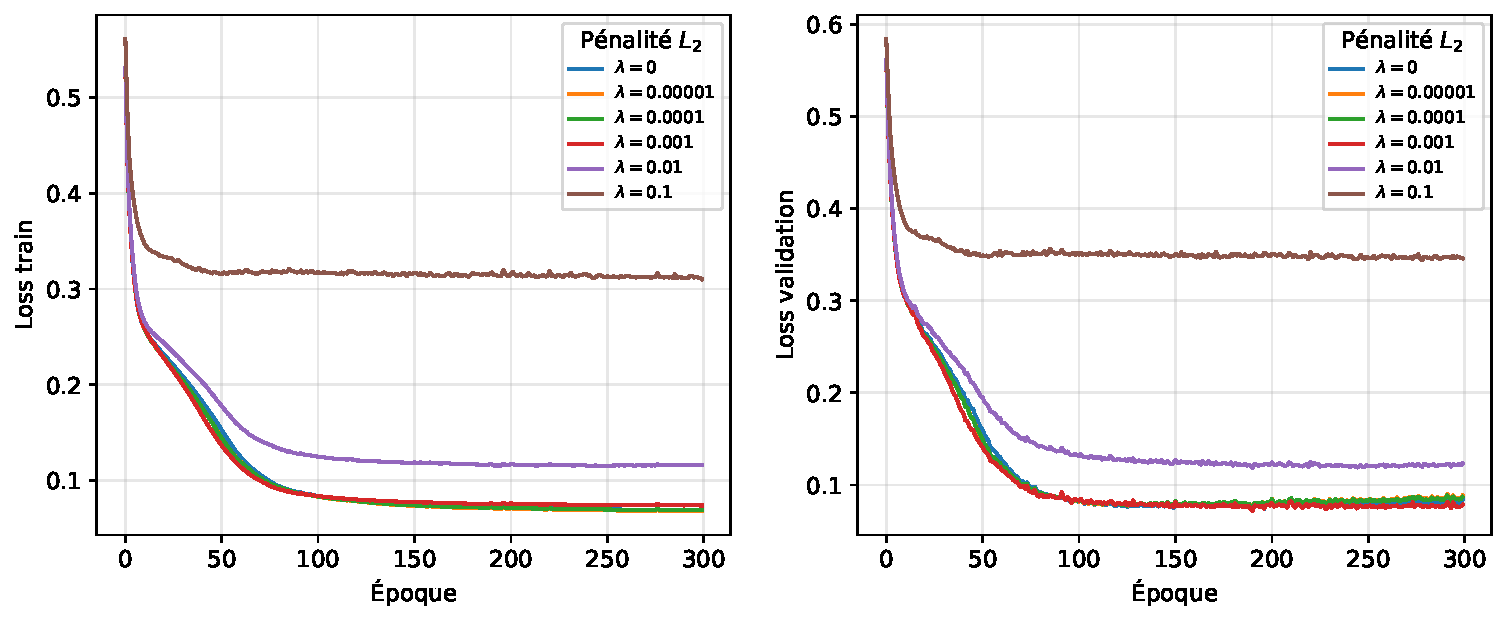
\includegraphics[width=\textwidth]{d_l2_loss.pdf}\\[4pt]
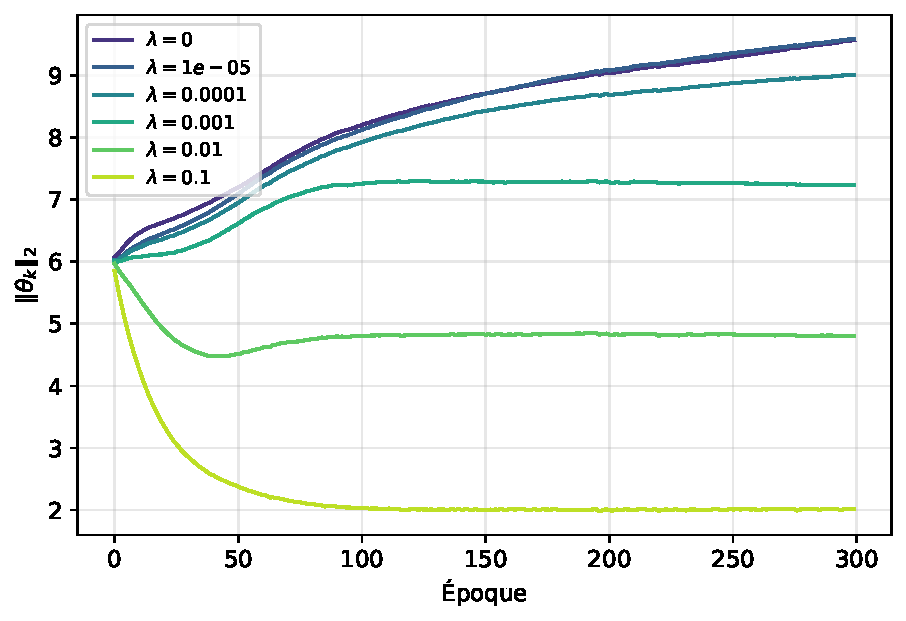
\includegraphics[width=0.62\textwidth]{d_l2_norm.pdf}
\caption{Effet de $\lambda$ : loss train et validation (haut) ; norme $\norm{\theta_k}_2$ au cours de l'entraînement (bas).}
\label{fig:d_l2}
\end{figure}

\subsection{Dropout}

Pendant l'entraînement, chaque neurone caché est conservé avec probabilité $p$ et sa sortie est rescalée en $\frac{M_j}{p} h_j$ ; en validation et en test, le dropout est désactivé. Le tableau~\ref{tab:d_dropout} et la figure~\ref{fig:d_dropout} montrent les résultats pour $p \in \{0{,}9, 0{,}8, 0{,}7, 0{,}5\}$.

Le dropout ralentit l'entraînement (la loss train finale croît de $0{,}0687$ sans dropout à $0{,}0724$ avec $p = 0{,}9$, et jusqu'à $0{,}1770$ avec $p = 0{,}5$) et dégrade légèrement la loss de validation à budget d'époques constant : $0{,}0929$ pour $p = 0{,}9$ contre $0{,}0842$ sans dropout. C'est attendu sur ce problème de petite dimension : avec seulement $900$ exemples et un réseau déjà modeste, le sur-apprentissage à $300$ époques est faible, donc le dropout ajoute surtout du bruit d'estimation. Le modèle sélectionné sur validation est $p = 0{,}9$ ; à taux trop élevé ($\delta = 0{,}5$), le réseau sous-apprend (accuracy $0{,}913$). Il est intéressant de noter que le dropout $p = 0{,}9$ produit finalement la meilleure accuracy de \emph{test} du protocole ($0{,}963$, tableau~\ref{tab:d_test}) : son effet régularisant, même léger, est positif hors échantillon.

\begin{figure}[H]
\centering
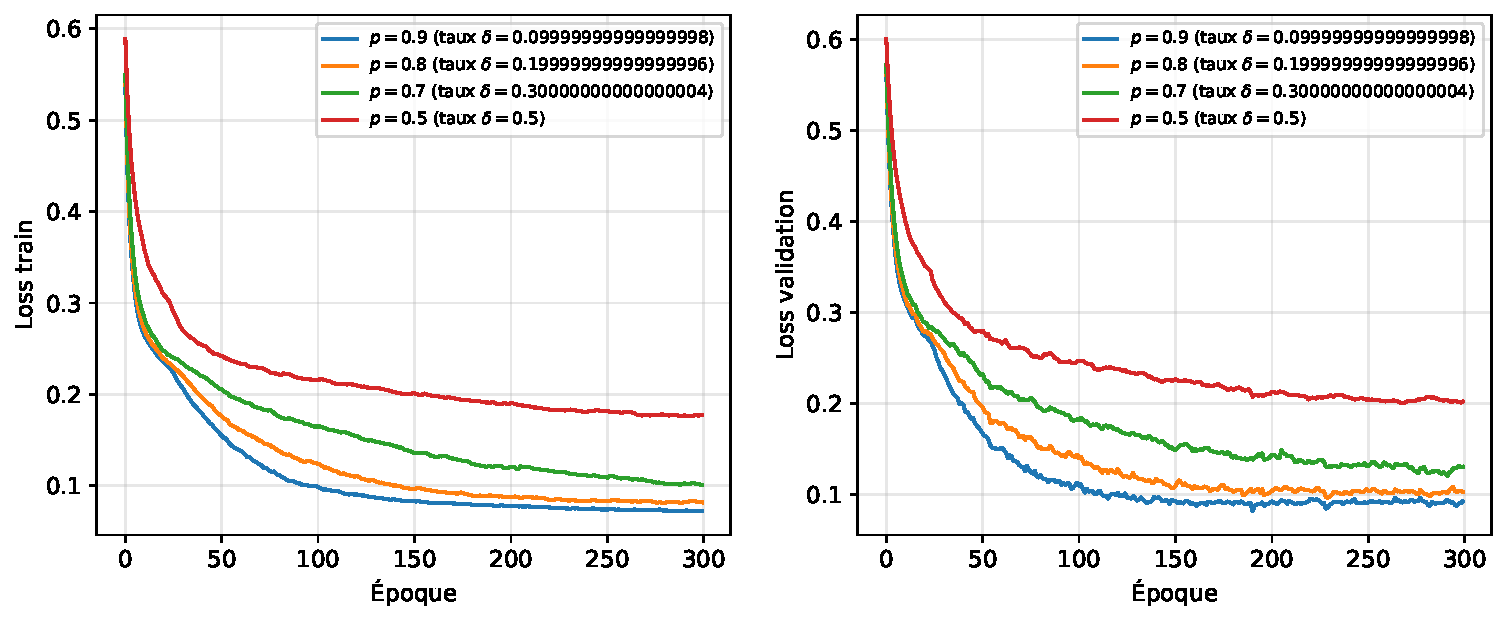
\includegraphics[width=\textwidth]{d_dropout.pdf}
\caption{Effet du taux de conservation $p$ du dropout : loss train (gauche) et validation (droite).}
\label{fig:d_dropout}
\end{figure}

\subsection{Early stopping}

Après chaque époque, la loss de validation est calculée, les meilleurs paramètres sont sauvegardés, un compteur est incrémenté si la validation ne s'améliore pas, et l'entraînement s'arrête après $P = 20$ époques sans amélioration, en restaurant les meilleurs paramètres. La figure~\ref{fig:d_early} montre que l'early stopping sélectionne l'époque $126$, avec une loss de validation de $0{,}0762$ --- la \emph{meilleure} loss de validation de toute l'étude --- et une norme de paramètres de $8{,}50$, plus faible que celle du modèle non régularisé ($9{,}57$). L'early stopping agit donc comme une régularisation implicite : il stoppe l'entraînement avant que les poids ne croissent excessivement.

\begin{figure}[H]
\centering
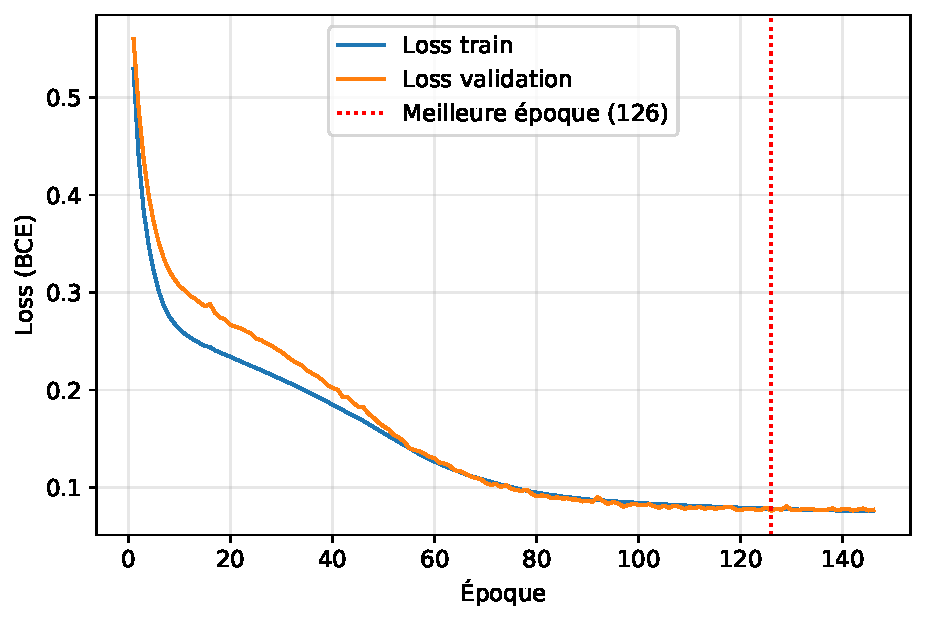
\includegraphics[width=0.62\textwidth]{d_early.pdf}
\caption{Early stopping (patience 20) : l'entraînement s'arrête à l'époque 126, au minimum de la loss de validation.}
\label{fig:d_early}
\end{figure}

\subsection{Sélection par validation et évaluation finale sur test}

Le protocole est strict : pour chaque famille de régularisation, le meilleur hyperparamètre est choisi sur la validation, puis le modèle sélectionné est évalué \emph{une seule fois} sur le test. Le tableau~\ref{tab:d_test} présente cette évaluation finale. Les quatre modèles atteignent une accuracy de test comparable ($0{,}957$ à $0{,}963$), le dropout $p = 0{,}9$ étant le meilleur en accuracy ($0{,}963$) et l'early stopping le meilleur en loss de validation. La figure~\ref{fig:boundary} montre la frontière de décision du modèle sélectionné, qui épouse correctement la géométrie des deux croissants.

\begin{figure}[H]
\centering
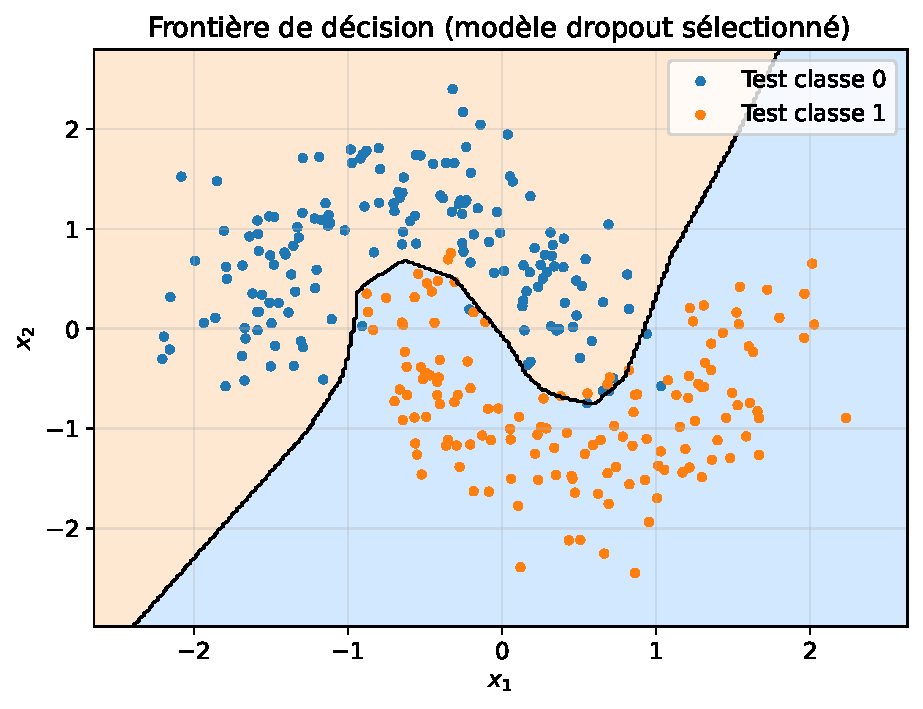
\includegraphics[width=0.6\textwidth]{d_boundary.pdf}
\caption{Frontière de décision du modèle sélectionné (dropout $p = 0{,}9$) sur le jeu de test.}
\label{fig:boundary}
\end{figure}

\section{Optimisation sous contraintes}
\label{sec:constraints}

\subsection{De la pénalité à la contrainte explicite}

La régularisation $L_2$ résout $\min_\theta F_{\mathrm{train}}(\theta) + \frac{\lambda}{2} \norm{\theta}_2^2$. On étudie maintenant la formulation sous contrainte :
\[
\min_{\theta} \; F_{\mathrm{train}}(\theta)
\qquad \text{s.c.} \qquad
\norm{\theta}_2 \le R,
\qquad
\norm{\theta}_2^2 = \sum_{\ell} \norm{\vect{W}^{(\ell)}}_F^2 ,
\]
les biais étant exclus de la contrainte, comme pour la pénalité.

\subsection{Projection sur la boule euclidienne}

Pour $\mathcal{C} = \{\theta : \norm{\theta}_2 \le R\}$, la projection euclidienne a une forme explicite :
\[
P_{\mathcal{C}}(z) =
\begin{cases}
z & \text{si } \norm{z}_2 \le R,\\[2pt]
R \, \dfrac{z}{\norm{z}_2} & \text{si } \norm{z}_2 > R.
\end{cases}
\]
Dans le code, cette projection est appliquée globalement à l'ensemble des poids $\{\vect{W}^{(\ell)}\}_{\ell}$ (les biais restant libres), ce qui revient à un rescaling uniforme de tous les poids par le facteur $\min\bigl(1, R/\norm{\theta}_2\bigr)$.

\subsection{Gradient projeté}

La méthode de gradient projeté consiste à alterner un pas d'optimiseur non contraint et la projection :
\[
\tilde{\theta}_{k+1} = \theta_k - \alpha_k \nabla F_{\mathcal{B}_k}(\theta_k),
\qquad
\theta_{k+1} = P_{\mathcal{C}}\bigl(\tilde{\theta}_{k+1}\bigr).
\]
L'implémentation (\texttt{constraints.py}) est générique : la classe \texttt{ProjectedOptimizer} enveloppe n'importe quel optimiseur de base (SGD, Momentum ou Adam) et projette après chaque mise à jour. Elle enregistre aussi le résidu de faisabilité avant projection,
\[
r_{\mathrm{feas}}(k) = \max\bigl(0, \norm{\tilde{\theta}_{k+1}}_2 - R\bigr),
\]
afin de visualiser à quel point la contrainte mord sur l'itération.

\subsection{Influence du rayon $R$}

La référence non contrainte (Adam, $300$ époques) fournit $R_0 = \norm{\theta^\star}_2 = 9{,}572$. Le tableau~\ref{tab:e} et la figure~\ref{fig:e_norm} présentent les résultats pour $R \in \{0{,}5R_0,\ 0{,}75R_0,\ R_0,\ 1{,}5R_0,\ 2R_0\}$.

Pour $R \ge 1{,}5R_0$, la contrainte est \emph{inactive} : le gradient projeté coïncide exactement avec l'entraînement non contraint (mêmes pertes, même norme finale, zéro projection). Pour $R = R_0$, la contrainte ne devient active qu'en toute fin d'entraînement (4 projections sur les $8700$ pas, norme finale $9{,}571$ contre $R = 9{,}572$) : c'est cohérent, puisque $R_0$ est par construction la norme de la solution non contrainte. Pour $R = 0{,}75R_0$, la contrainte est active pendant tout l'entraînement ($6955$ projections) et la norme finale sature exactement à $R = 7{,}179$ : la perte de validation remonte légèrement à $0{,}0855$, mais l'accuracy reste à $0{,}977$ --- le réseau supporte une réduction de $25\,\%$ de la norme de ses poids sans perte de performance. Pour $R = 0{,}5R_0$, la contrainte est trop sévère : loss de validation $0{,}2138$, accuracy $0{,}913$ : le réseau n'a plus assez de capacité pour ajuster les données. Diminuer $R$ contraint donc le modèle de façon monotone : d'abord sans effet (contrainte inactive), puis avec une légère perte (contrainte active mais tolérable), puis avec une dégradation nette (sous-apprentissage).

\begin{figure}[H]
\centering
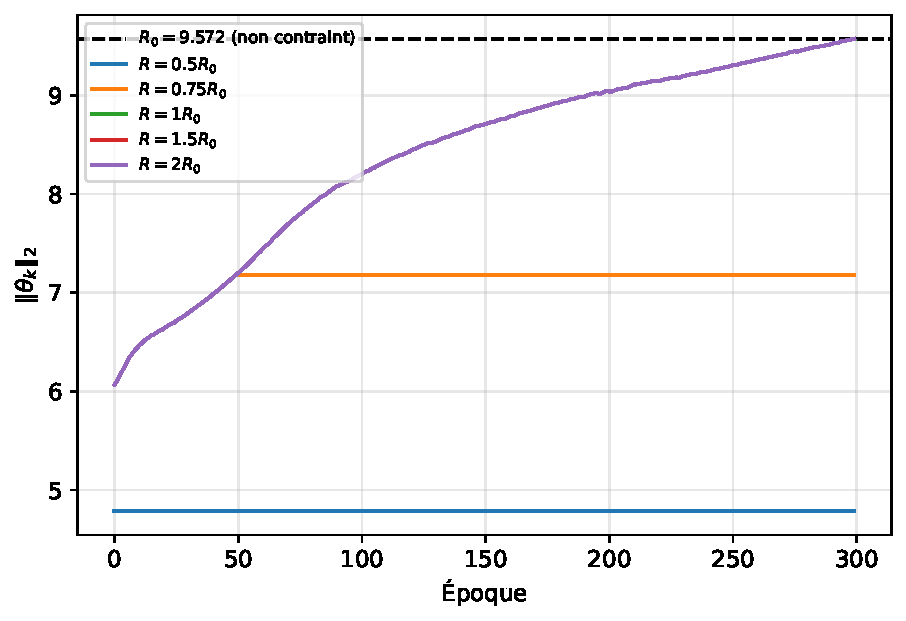
\includegraphics[width=0.62\textwidth]{e_norm.pdf}\\[4pt]
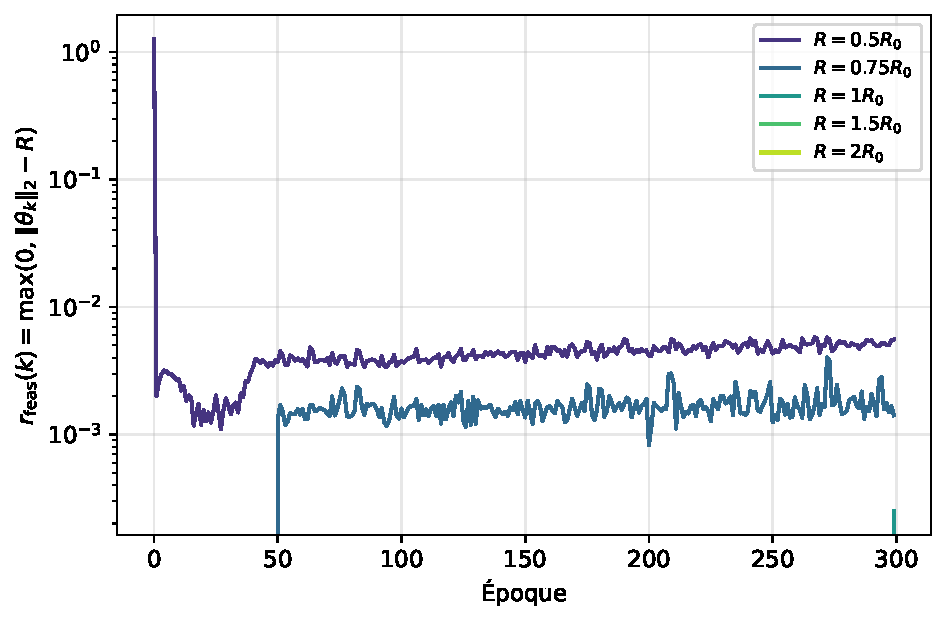
\includegraphics[width=0.62\textwidth]{e_rfeas.pdf}
\caption{Gradient projeté : évolution de $\norm{\theta_k}_2$ (haut) et du résidu de faisabilité $r_{\mathrm{feas}}(k)$ (bas) pour différents rayons $R$.}
\label{fig:e_norm}
\end{figure}

\subsection{Comparaison pénalisation $L_2$ / contrainte explicite}

La question centrale de la partie F est : \emph{régulariser par une pénalité ou imposer directement une contrainte ?} Pour comparer rigoureusement les deux formulations, on construit des couples $(\lambda, R)$ produisant des normes finales comparables : pour chaque $\lambda \in \{10^{-4}, 10^{-3}, 10^{-2}\}$, on relève la norme $\norm{\theta^\star}_2$ obtenue par la solution pénalisée, puis on entraîne le modèle contraint avec $R$ égal à cette norme (3 graines d'initialisation par configuration). Le tableau~\ref{tab:f} et la figure~\ref{fig:f_pair} résument la comparaison.

Pour un rayon lâche ($R = 9{,}009$, couple avec $\lambda = 10^{-4}$), les deux approches sont équivalentes : loss de validation $0{,}0828$ contre $0{,}0806$, accuracy de test $0{,}960$ dans les deux cas, et écart-type entre graines comparable. Pour un rayon moyen ($R = 7{,}232$, couple avec $\lambda = 10^{-3}$), les performances restent proches ($0{,}0794$ contre $0{,}0870$ en loss de validation ; $0{,}959$ contre $0{,}961$ en accuracy de test). En revanche, pour un rayon serré ($R = 4{,}805$, couple avec $\lambda = 10^{-2}$), la contrainte explicite dégrade nettement plus la solution que la pénalité : loss de validation $0{,}2232$ contre $0{,}1233$, accuracy de test $0{,}910$ contre $0{,}950$.

\begin{figure}[H]
\centering
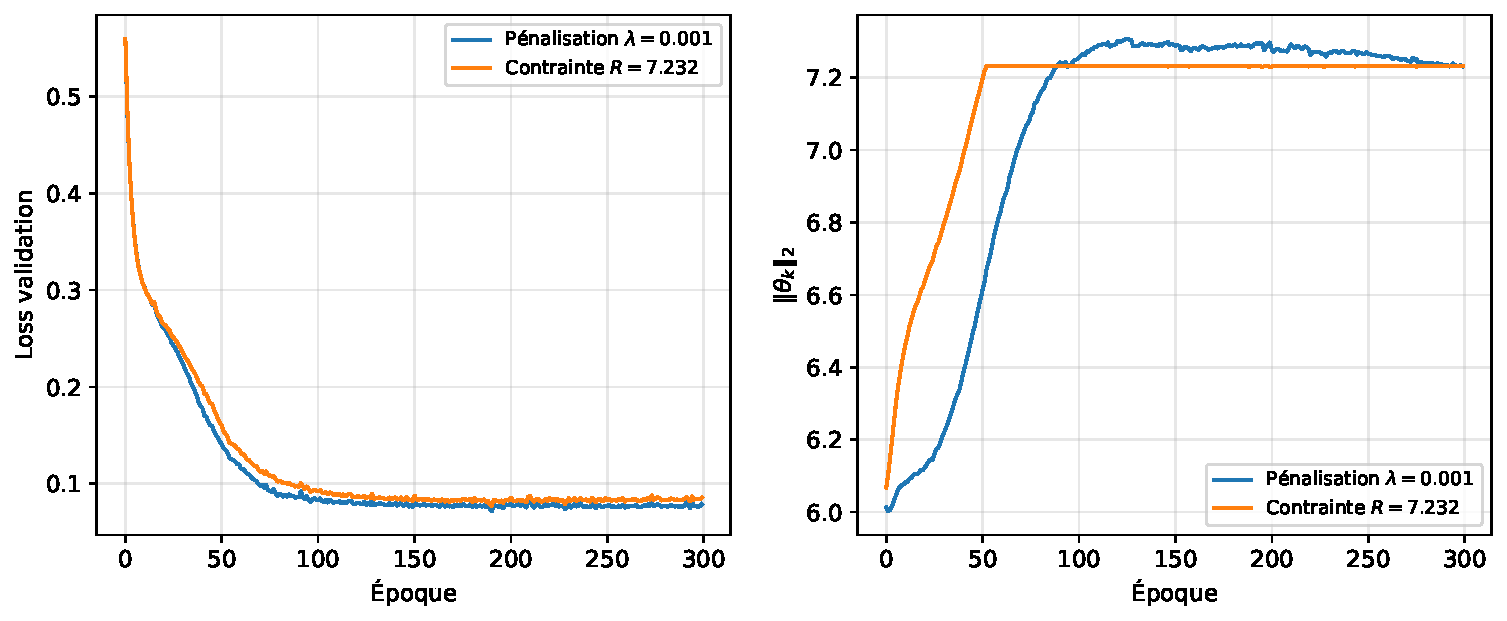
\includegraphics[width=\textwidth]{f_pair.pdf}
\caption{Couple $(\lambda = 10^{-3},\, R = 7{,}232)$ : loss de validation (gauche) et norme des poids (droite) pour la pénalisation et la contrainte explicite.}
\label{fig:f_pair}
\end{figure}

\textbf{Interprétation.} La différence de comportement à rayon serré s'explique par la géométrie des deux problèmes. La pénalité autorise la norme à osciller autour de sa valeur d'équilibre (solution intérieure du problème $F + \frac{\lambda}{2}\norm{\theta}^2$), et la répartition des poids entre les trois couches s'ajuste librement : la solution pénalisée finit à $\norm{\theta^\star} = 4{,}837$, légèrement au-dessus du $R$ de référence, avec une répartition des poids dictée par le gradient. La contrainte, elle, maintient $\theta$ \emph{exactement sur la frontière} de la boule ($\norm{\theta} = R$ à chaque itération une fois la contrainte active), c'est-à-dire sur un ensemble de mesure nulle : le gradient projeté redistribue alors les poids par un rescaling uniforme après chaque pas, indépendamment de l'importance de chaque couche. Sur ce problème non convexe, ces deux chemins conduisent à des minima locaux différents, et le minimum trouvé par la pénalisation généralise mieux. Ce résultat illustre un point méthodologique important : dans un problème non convexe, \emph{il n'existe pas de correspondance simple} $\lambda \leftrightarrow R$ garantissant des solutions identiques, ce qui est précisément l'objet de l'indication du sujet.

\section{Vérification avec PyTorch}
\label{sec:torch}

Une fois les implémentations NumPy validées, une architecture strictement équivalente est construite sous PyTorch (\texttt{torch\_verify.py}) : mêmes dimensions ($2 \to 16 \to 8 \to 1$, ReLU + sigmoïde), mêmes poids initiaux (recopiés du modèle NumPy), mêmes mini-batchs (indices générés par le même générateur NumPy) et mêmes hyperparamètres, le tout en double précision (float64) pour isoler l'erreur de l'implémentation. Le tableau~\ref{tab:g} et la figure~\ref{fig:torch} comparent \texttt{SGD} $\leftrightarrow$ \texttt{torch.optim.SGD} et \texttt{Adam} $\leftrightarrow$ \texttt{torch.optim.Adam}.

\begin{figure}[H]
\centering
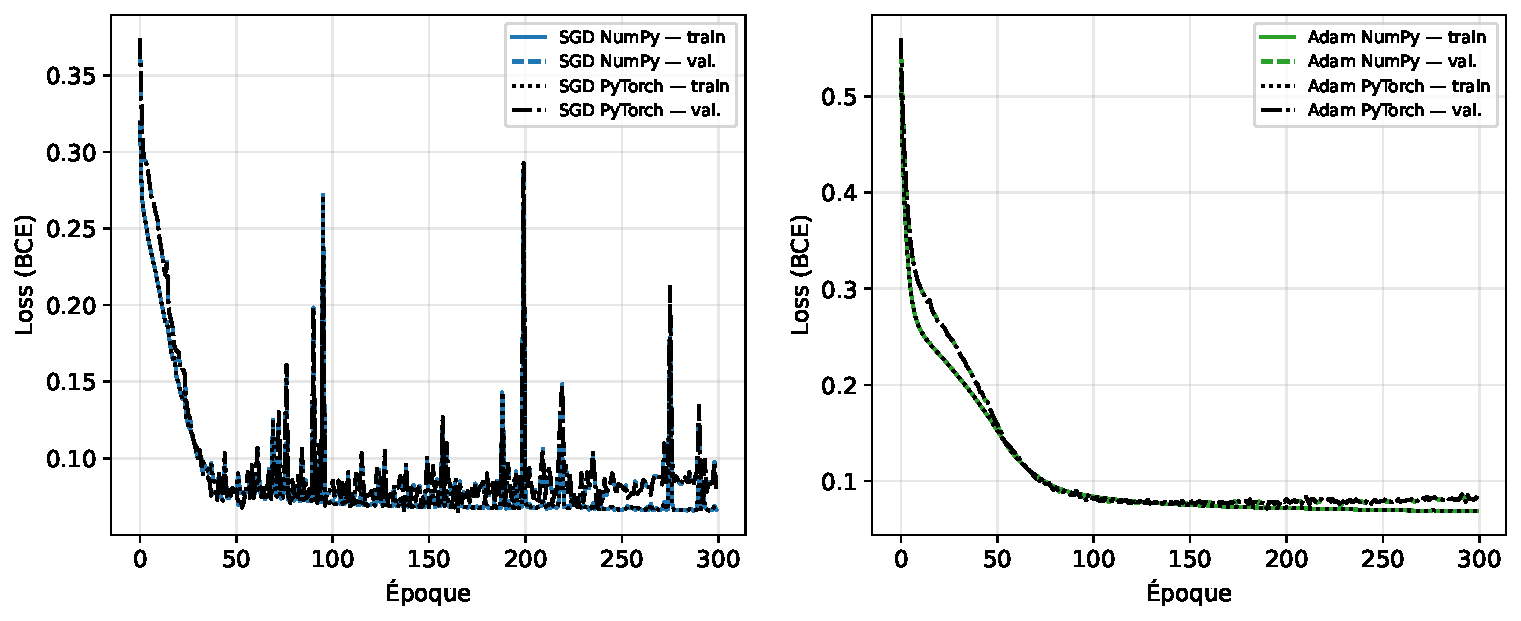
\includegraphics[width=\textwidth]{g_torch.pdf}
\caption{NumPy contre PyTorch : les courbes de loss sont superposées (écart maximal de $5{,}7\times10^{-11}$ pour SGD et $1{,}1\times10^{-12}$ pour Adam).}
\label{fig:torch}
\end{figure}

Les écarts maximaux entre les losses sont de $5{,}7 \times 10^{-11}$ (SGD) et $1{,}1 \times 10^{-12}$ (Adam), c'est-à-dire du niveau de l'arrondi en double précision ; les accuracies de validation et de test sont identiques. Les implémentations NumPy sont donc numériquement équivalentes aux implémentations de référence de PyTorch.

\section{Protocole expérimental}
\label{sec:protocole}

Le protocole respecte les exigences du sujet :
\begin{enumerate}
  \item graines fixées partout (données, découpage, initialisation, mini-batchs) ;
  \item même découpage et même architecture dans toutes les expériences comparables ;
  \item toutes les valeurs d'hyperparamètres documentées (taux d'apprentissage, $\beta_1, \beta_2$, $\lambda$, $p$, $P$, $R$) ;
  \item sélection des hyperparamètres sur la validation uniquement ;
  \item jeu de test consulté uniquement après sélection finale (tableau~\ref{tab:d_test}), sauf dans les expériences où le sujet le demande explicitement (parties F et G) ;
  \item répétition des expériences stochastiques sur 3 graines ($42$, $7$, $123$) avec moyennes et écarts-types ;
  \item enregistrement systématique de la loss train/validation, de $\norm{\nabla F(\theta_k)}$, de $\norm{\theta_k}_2$, de l'accuracy et, pour les expériences sous contraintes, de $r_{\mathrm{feas}}(k)$.
\end{enumerate}
L'exécution de \texttt{python main.py} rejoue l'intégralité du protocole et régénère toutes les figures et tous les tableaux du rapport.

\section{Discussion critique}
\label{sec:discussion}

\subsection{Réponses aux questions scientifiques}
\label{sec:questions}

\begin{enumerate}
  \item \textbf{Quel optimiseur converge le plus rapidement ?} SGD et Momentum (accuracy de validation $\ge 0{,}95$ atteinte en $18{,}7 \pm 5{,}2$ et $17{,}7 \pm 3{,}3$ époques), nettement devant Adam avec $\alpha = 10^{-3}$ ($47{,}3 \pm 11{,}9$ époques), dont les premiers pas sont petits.
  \item \textbf{Quel optimiseur produit la meilleure performance de validation ?} Adam : loss de validation $0{,}0821$ et accuracy $0{,}977$, légèrement meilleur que SGD ($0{,}0847$ ; $0{,}974$).
  \item \textbf{Le meilleur résultat d'entraînement correspond-il au meilleur résultat de test ?} Pas exactement : SGD minimise le plus la loss train ($0{,}0667$) et obtient la meilleure accuracy de test ($0{,}967$, partie G), tandis qu'Adam, meilleur en validation, obtient $0{,}957$ en test. Le classement train, validation et test ne coïncident donc pas ; les écarts ($\approx 1$ point) sont du même ordre que la variabilité entre graines.
  \item \textbf{À partir de quelle époque observe-t-on du sur-apprentissage ?} Vers l'époque $\approx 190$ : la loss de validation, minimale à l'époque $191$ ($0{,}0714$), remonte ensuite alors que la loss train continue de décroître ; à $300$ époques l'écart train/validation vaut $0{,}016$ et il atteint $0{,}192$ à $2000$ époques.
  \item \textbf{Quel effet produit $L_2$ sur $\norm{\theta}$ et sur l'écart train/validation ?} $\norm{\theta^\star}_2$ décroît de façon monotone avec $\lambda$ ($9{,}57$ sans pénalité, $7{,}23$ à $\lambda = 10^{-3}$, $2{,}02$ à $\lambda = 0{,}1$). L'écart validation$-$train est réduit de $0{,}016$ à $0{,}005$ à $\lambda^\star = 10^{-3}$ ; au-delà de $10^{-2}$, le modèle sous-apprend.
  \item \textbf{Quel effet produit le dropout ?} Il ralentit l'entraînement et augmente légèrement la loss de validation à budget d'époques constant, mais le modèle sélectionné ($p = 0{,}9$) obtient la meilleure accuracy de test ($0{,}963$). Un taux trop élevé ($\delta = 0{,}5$) dégrade fortement les performances.
  \item \textbf{Quel modèle est sélectionné par early stopping ?} Celui de l'époque $126$, de loss de validation $0{,}0762$ (la meilleure de l'étude) et de norme $8{,}50 < 9{,}57$, illustration de la régularisation implicite apportée par l'arrêt précoce.
  \item \textbf{Quel effet produit une diminution de $R$ ?} Rien tant que $R \ge R_0$ (contrainte inactive) ; à $0{,}75R_0$, la contrainte est active, la norme sature à $R$ et la loss de validation remonte légèrement ($0{,}0855$, accuracy inchangée $0{,}977$) ; à $0{,}5R_0$, dégradation nette (accuracy $0{,}913$).
  \item \textbf{Dans quelles expériences la contrainte est-elle active ?} Active (projections effectives à chaque époque) pour $R = 0{,}5R_0$ et $R = 0{,}75R_0$ ; quasi active en fin d'entraînement pour $R = R_0$ ; inactive pour $R \ge 1{,}5R_0$. Dans la partie F, la contrainte est active pour les trois couples $(\lambda, R)$ étudiés.
  \item \textbf{Quelle différence entre pénalisation $L_2$ et contrainte $\norm{\theta} \le R$ ?} À normes finales comparables, les deux approches sont équivalentes pour les rayons lâches et moyens ; pour un rayon serré ($R = 4{,}81$), la contrainte dégrade nettement plus la solution (loss de validation $0{,}223$ contre $0{,}123$ ; accuracy de test $0{,}910$ contre $0{,}950$), car elle maintient $\theta$ sur la frontière de la boule par rescaling uniforme, alors que la pénalité laisse la répartition des poids s'ajuster selon le gradient.
  \item \textbf{Les résultats NumPy et PyTorch sont-ils cohérents ?} Oui, à $10^{-11}$ près sur les pertes (écart de l'ordre de l'arrondi float64), avec des accuracies identiques.
  \item \textbf{Quelles limites méthodologiques ?} Voir ci-dessous.
\end{enumerate}

\subsection{Limites méthodologiques}

\begin{itemize}
  \item \textbf{Problème simple} : \texttt{make\_moons} à $2$ dimensions est presque saturé par tous les modèles (accuracy $\approx 0{,}96$) ; les écarts entre méthodes sont faibles et proches du bruit entre graines. Un problème plus difficile (images, plus de classes) discriminerait mieux les techniques.
  \item \textbf{Une seule architecture et un seul découpage} : les conclusions sont conditionnelles à $2 \to 16 \to 8 \to 1$ et au découpage $60/20/20$ ; une étude croisée (plusieurs architectures, validation croisée) serait plus robuste.
  \item \textbf{Optimisation non convexe} : chaque entraînement atteint un minimum local potentiellement différent ; les comparaisons pénalisation/contrainte restent donc qualitatives, sans correspondance théorique $\lambda \leftrightarrow R$ exacte.
  \item \textbf{Interaction Adam/projection} : le gradient projeté projette $\theta$ mais pas les moments $\vect{m}, \vect{v}$ d'Adam ; des méthodes dédiées (projected Adam, primal-dual) pourraient être plus efficaces à rayon serré.
  \item \textbf{Contrainte globale} : la contrainte porte sur l'ensemble des poids et non par couche ; une contrainte par couche pourrait répartir différemment la capacité.
  \item \textbf{Dropout et budget d'époques} : avec dropout, un budget d'époques plus grand serait nécessaire pour converger ; la comparaison à budget constant (300 époques) le désavantage.
  \item \textbf{Test partiellement réutilisé} : dans les parties F et G, le test a été utilisé pour la comparaison (explicitement demandé par le sujet), ce qui limite l'interprétation stricte de l'évaluation finale unique.
\end{itemize}

\section{Conclusion}

Le projet a suivi la chaîne logique complète : construire le réseau $f_\theta$ en NumPy (propagation avant, rétropropagation dérivée puis validée par gradient checking à $10^{-11}$ près), minimiser $F_{\mathrm{train}}(\theta)$ par SGD, Momentum et Adam comparés selon un protocole strict, contrôler la généralisation par $L_2$, dropout et early stopping avec sélection sur validation et évaluation unique sur test, puis imposer une contrainte explicite $\norm{\theta}_2 \le R$ résolue par gradient projeté, et enfin vérifier toute l'implémentation contre PyTorch. Les enseignements principaux sont les suivants. Sur ce problème, les trois optimiseurs convergent vers des performances comparables, la vitesse de convergence ne présage pas de la généralisation ; le sur-apprentissage apparaît vers l'époque $190$ et il est efficacement contenu par l'early stopping et par $\lambda = 10^{-3}$ ; une contrainte sur la norme des poids est sans effet tant qu'elle est inactive et devient un outil de contrôle précis de la complexité lorsqu'elle est active, au prix --- à rayon très serré --- d'une perte plus marquée que la pénalisation équivalente. Le projet a ainsi permis de comprendre non seulement \emph{quel} modèle fonctionne, mais \emph{pourquoi}, \emph{comment} il est optimisé, \emph{comment} sa généralisation est contrôlée et \emph{comment} les contraintes influencent son apprentissage.

\appendix
\section{Structure du code et reproduction}

Le dépôt contient :
\begin{verbatim}
project/
|-- data.py            # génération, split, standardisation
|-- layers.py          # Linear, ReLU, Sigmoid, Dropout
|-- model.py           # assemblage du réseau (MiniNet)
|-- losses.py          # BCE et gradient
|-- optimizers.py      # SGD, Momentum, Adam
|-- regularization.py  # pénalité L2, EarlyStopping
|-- constraints.py     # norme, projection L2, ProjectedOptimizer
|-- train.py           # boucle d'entraînement
|-- experiments.py     # protocoles A..G, tableaux LaTeX
|-- torch_verify.py    # vérification PyTorch
|-- plots.py           # courbes et visualisations
|-- main.py            # point d'entrée
|-- figures/           # figures générées (PDF)
|-- results/           # summary.json, tables.tex
|-- README.md
`-- rapport.tex / rapport.pdf
\end{verbatim}

\textbf{Dépendances} : Python 3.9+, NumPy, scikit-learn, matplotlib ; PyTorch (optionnel, pour la vérification de la partie G).

\textbf{Reproduction} : \texttt{python main.py} exécute toutes les expériences (environ 90 secondes) et régénère les figures et les tableaux utilisés dans ce rapport.

\begin{thebibliography}{9}
\bibitem{he2015} K.~He, X.~Zhang, S.~Ren, J.~Sun, \emph{Delving Deep into Rectifiers: Surpassing Human-Level Performance on ImageNet Classification}, ICCV 2015.
\bibitem{kingma2015} D.~P.~Kingma, J.~Ba, \emph{Adam: A Method for Stochastic Optimization}, ICLR 2015.
\bibitem{srivastava2014} N.~Srivastava et al., \emph{Dropout: A Simple Way to Prevent Neural Networks from Overfitting}, JMLR 2014.
\bibitem{bertsekas} D.~P.~Bertsekas, \emph{Nonlinear Programming}, Athena Scientific, 3\textsuperscript{e} éd., 2016 (gradient projeté).
\end{thebibliography}

\end{document}
